\chapter{No Camera}

\label{ch:no_camera}

\section{Introduction?? not sure about the name!!!}
HuddleLamp was a project that introduced some novel ideas such as the Hybrid sensing approach in tracking devices. It successfully initiated a discussion into spatially aware mobile devices. By utilising various technologies and devices they were able to bring the idea into fruition. 

However there are some drawbacks to the product, such as needing to carry around a laptop, a stand and a camera for the algorithm to work. The space that we could use, the canvas of the application, was limited by the area that was visible to the camera. This area is proportional to the height of the camera from the table. Another drawback noticed by \citeauthor{huddelamp-paper} was the noticeable delay between the physical movement of a screen and the corresponding reaction of the UI\cite{huddelamp-paper}. 

I am going to try and address some of these drawbacks by using a combination of BLE and Sensor fusion instead of a camera for my tracking and positioning system. I would be creating an Android application which means the computer would be unnecessary. It should also provide a better reaction time. 

I hope to make this into a library such that it would be easier to create applications to be used on the interactive table. Currently there is no clear documentation on how to create an application for HuddleLamp. By creating a library to work out the current location for the application and the scrolling on a screen, the majority of the complexity could be converted into a "black box" that the developers would not have to worry about. I plan to have a library that could cater to the needs of most developers. 

\begin{figure}[h]
  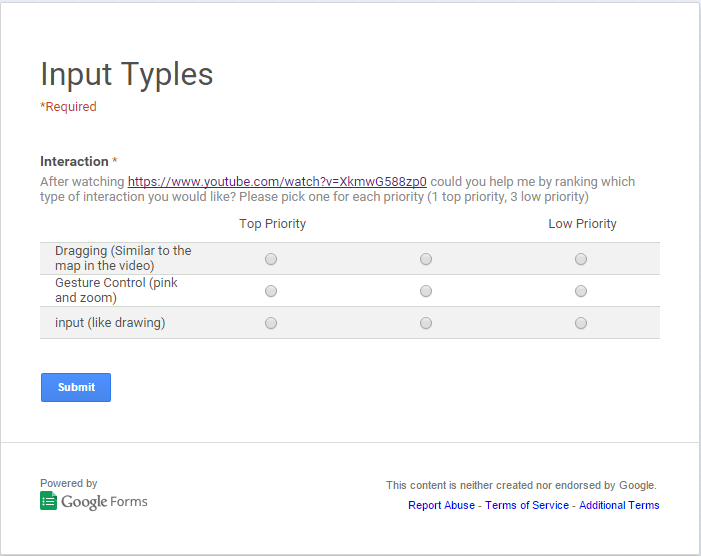
\includegraphics[scale=0.7]{images/googleform}
  \protect\caption{Form to find out preferred interactions} 
  \label{googleform}
\end{figure}